% !TeX program = xelatex
\documentclass{ctexart}
\usepackage[table]{xcolor}
\usepackage{template_by_mny}
\usepackage{float} 
\usepackage{listings}
\usepackage[figuresright]{rotating}
\lstset{basicstyle=\ttfamily, breaklines=true, frame=single}

\title{偏振实验报告}
\class{物理 32/物理 31}
\name{冯家琦/周方远}
\id{2023011338/2023011263}

\begin{document}

\maketitle

\section{引言}
本报告记录了使用偏振和3D电影技术套件进行的实验。这些实验旨在探索偏振原理、3D成像技术及其应用。
\section{实验原理}
\section{实验仪器}
\section{实验步骤}
\subsection{Part1:偏振实验}

\subsubsection{实验1:马吕斯定律}
\begin{enumerate}
    \item 在激光器前放置一个偏振片。将其定位,使得透过的光亮度最大化。现在在光束路径中放置第二个偏振片,并将光电探测器放在它后面。以你选择的增量大小旋转第二个偏振片,并记录光电探测器上的电压值。
\end{enumerate}

\subsubsection{实验2:测量激光的偏振状态}
\begin{enumerate}
    \item 在激光器前放置一个偏振片。光电探测器再次放置在偏振片后面。现在以你选择的增量大小旋转偏振片,并测量光电探测器上的电压。
\end{enumerate}

\subsubsection{实验3:确定 $\lambda/4$ 板的取向}
\begin{enumerate}
    \item 将板放置在两个垂直的偏振片之间,并寻找透射最大值以确定 $\lambda/4$ 板的 45° 取向。
\end{enumerate}

\subsubsection{实验4:$\lambda/4$ 板对绿光的行为}
首先在激光器前放置一个偏振片,然后在其前面放置 $\lambda/4$ 板。$\lambda/4$ 板应相对于偏振片调整至 45°。现在证明绿激光在通过 $\lambda/4$ 板后变为圆偏振光。
\begin{figure}[H]
    \centering
    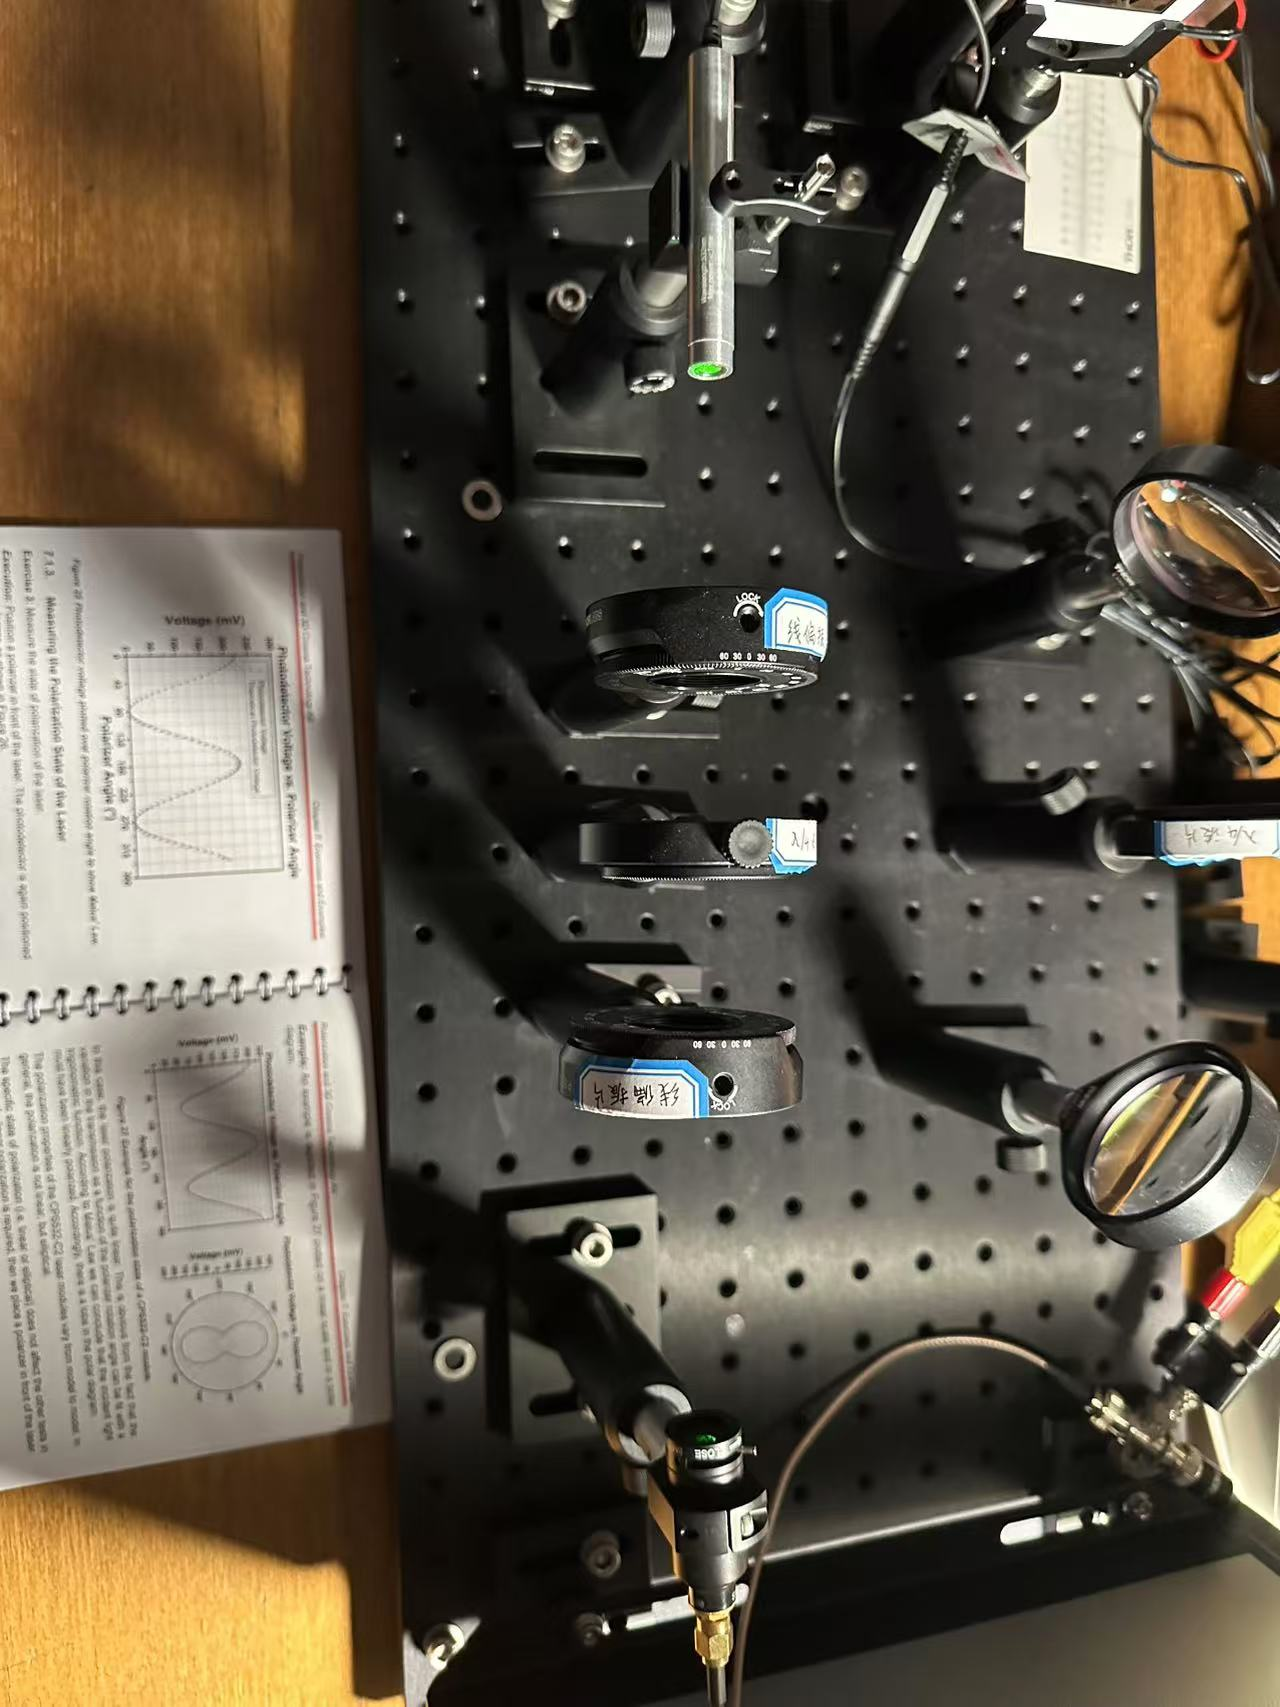
\includegraphics[width=0.3\textwidth]{偏振光路.jpg}
    \caption{实验4光路}
\end{figure}
调整第二个偏振器的角度,测量并记录对应的光强如下图所示
\begin{figure}[H]
    \centering
    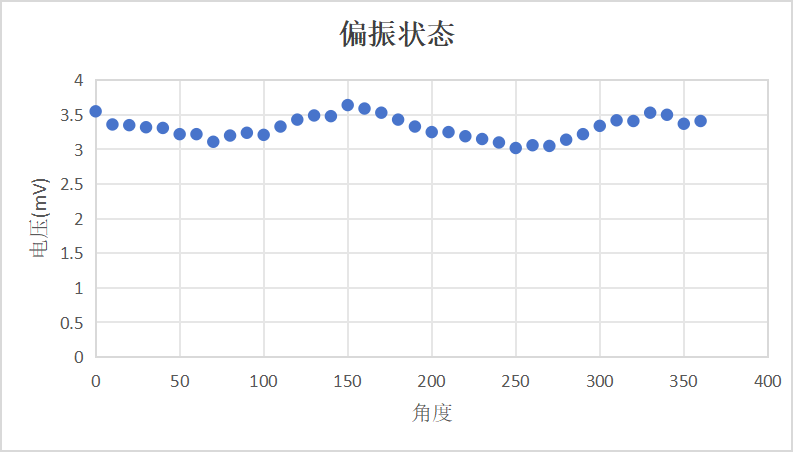
\includegraphics[width=0.5\textwidth]{实验5.png}
    \caption{实验5光强}
\end{figure}
可以看出,随着角度的变化,光强几乎不变

\subsubsection{实验5:糖量测定}
通过测量线性偏振光通过糖溶液时的偏振旋转角度,确定比例常数。

先在激光器前放两个相互垂直的线偏振片,然后在它们中间放一个玻璃容器,光路如图。
\begin{figure}[H]
    \centering
    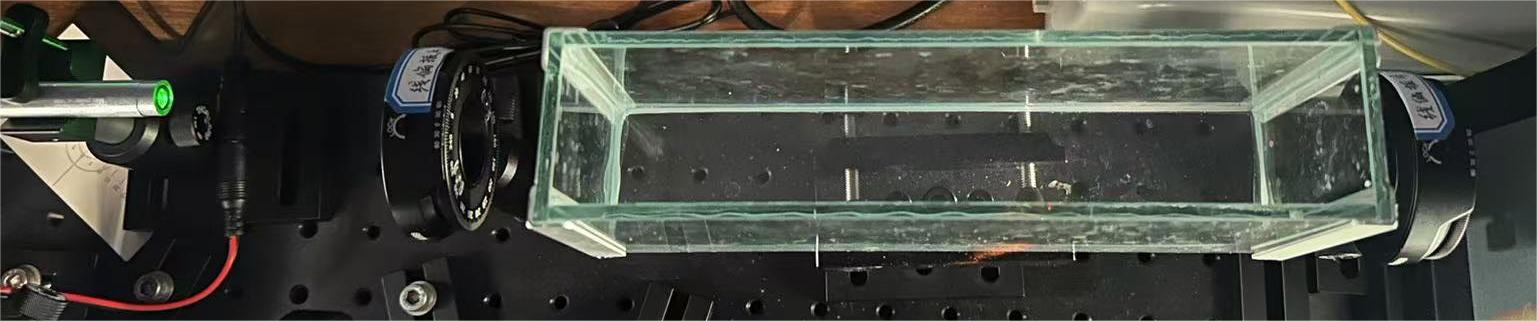
\includegraphics[width=0.7\textwidth]{糖光路(1).jpg}
    \caption{实验5光路}
\end{figure}
通过秤秤出22g糖并加入玻璃容器中,加入72mL水溶解。调整偏振片的角度使得光可以透过偏振片进入接受器,记录此时的角度。接下来如下图逐渐稀释糖溶液,记录每次稀释后的角度。
\begin{figure}[H]
    \centering
    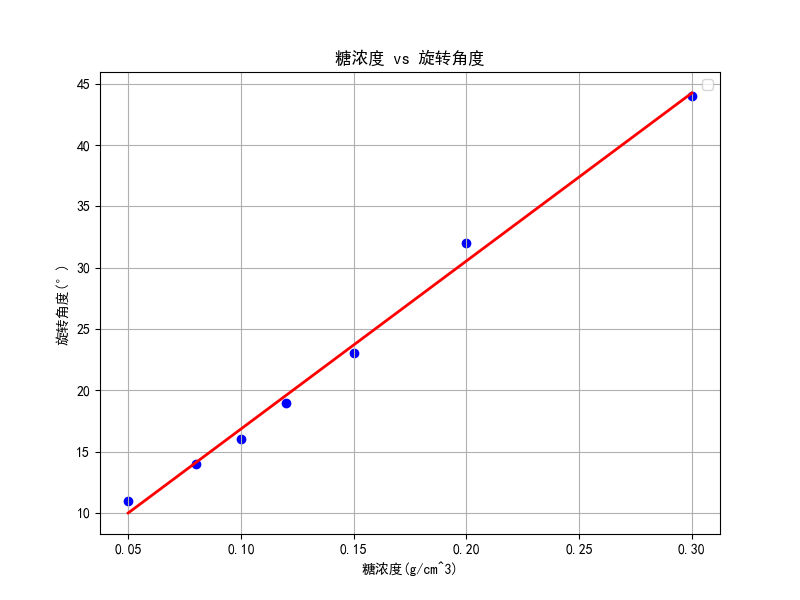
\includegraphics[width=0.5\textwidth]{糖浓度 vs 旋转角度.png}
\end{figure}
\end{document}